\documentclass[10pt]{article}
\usepackage{graphicx}
\usepackage{commath}
\usepackage{gensymb}
\usepackage{amsmath,amsfonts,amssymb}
\usepackage[none]{hyphenat}
\usepackage{listings}
\usepackage[english]{babel}
\usepackage{caption} 
\usepackage{hyperref}
\usepackage{booktabs}
\usepackage{array}
\usepackage{listings}
\lstset{
  frame=single,
  breaklines=true
}

\title{VECTORS}
\author{prasad deva}

\begin{document}

\maketitle


\section{10$^{th}$ Maths - Chapter 10}

This is Problem-3 from Exercise 10.3

\begin{enumerate}
\item Find the projection of the vector $\hat{i}-\hat{j}$ on the vector $\hat{i}+\hat{j}$  :
\end{enumerate}
\section{SOLUTION}
Taken points are $A=(1,-1), B=(1, 1)$  
\bigskip

The formula of the projection vector : $\frac{A^t\times B}{\norm B^2}\times B$
\bigskip

Find the projection vector:
\bigskip

$A^t\times B = (1, -1)\times \left(\begin{matrix}
1\\
1\\
\end{matrix}\right)  = (1\times1)+(1\times-1)=0$
\bigskip

$\norm B^2 = (B^t\times B)=(1,1)\left(\begin{matrix}
1\\
1\\
\end{matrix}\right)= (1\times1)+(1\times1)=2$
 \bigskip
 
projection vector = $\frac{A^t\times B}{\norm B^2}\times B$
\bigskip

   =$\frac{0}{2}\times \left(\begin{matrix}
   1\\
   1\\
   \end{matrix}\right)$
  \bigskip

    =(0,0)
\bigskip

projection vector = (0,0)

\begin{figure}[h]
  \centering
  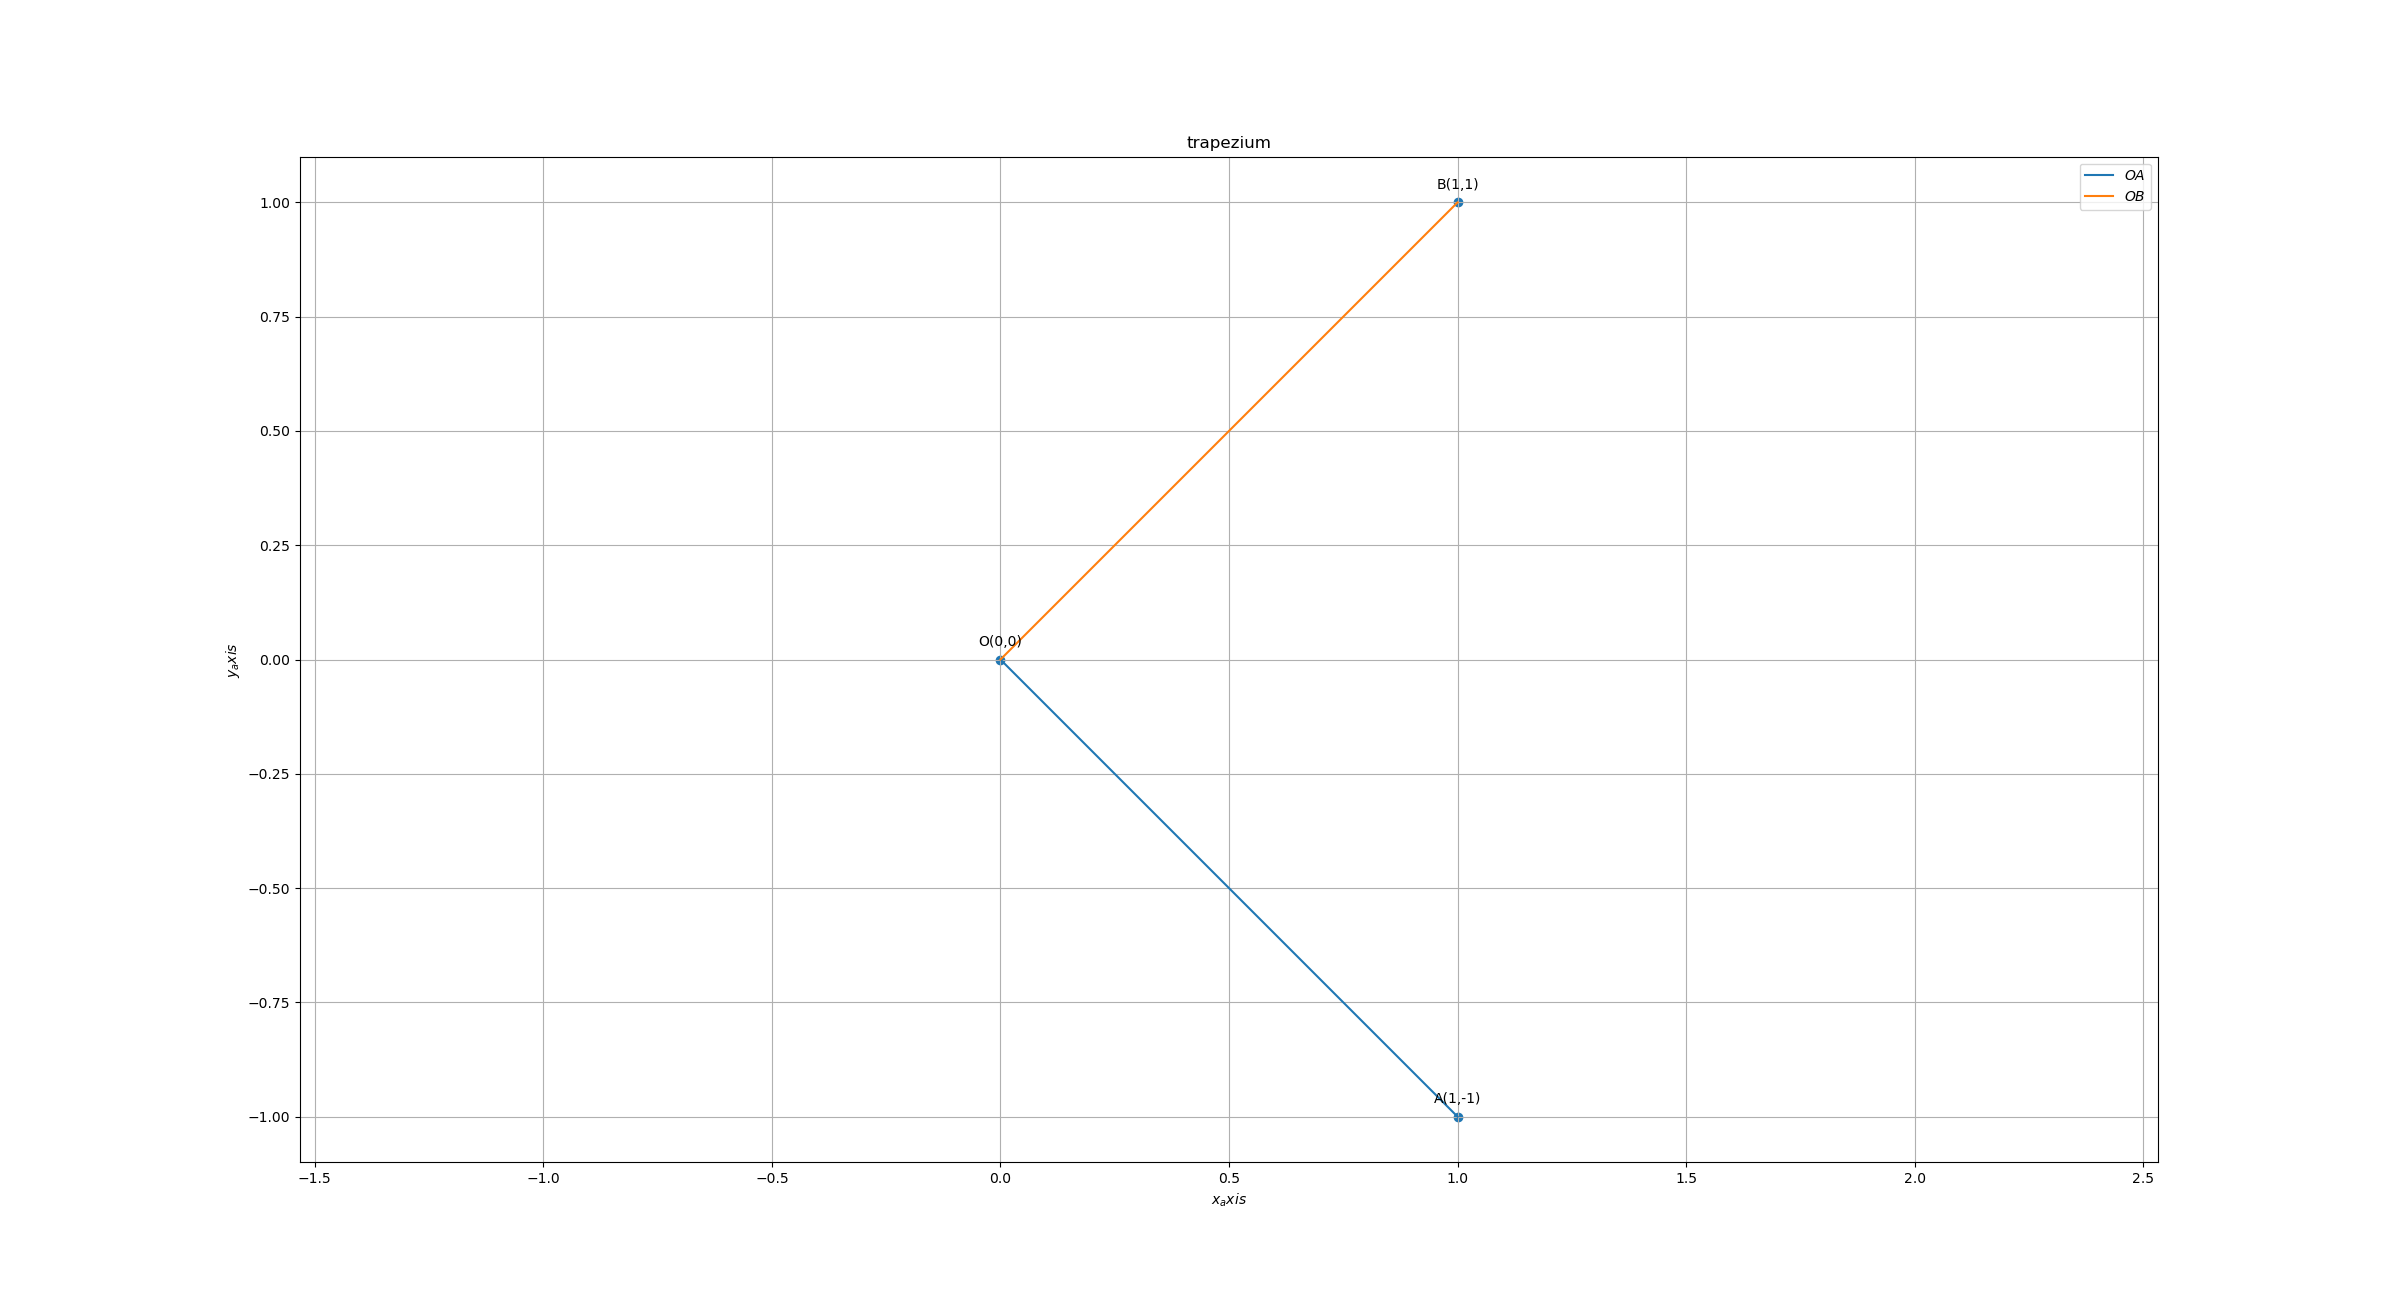
\includegraphics[scale=0.2]{vector.png}
\caption{}
\end{figure}

\end{document}
